\documentclass{article}
\usepackage{tikz}

\begin{document}

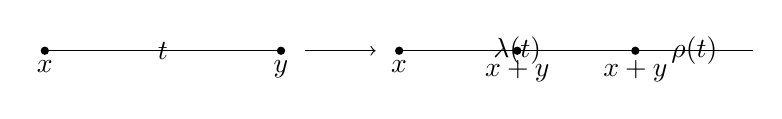
\begin{tikzpicture}[scale=1.5]
    % Draw the first line segment
    \draw (0,0) -- (2,0);
    \fill (0,0) circle (1pt) node[below] {$x$};
    \fill (2,0) circle (1pt) node[below] {$y$};
    \node at (1,0) {$t$};

    % Draw the arrow
    \draw[->] (2.2,0) -- (2.8,0);

    % Draw the second line segment
    \draw (3,0) -- (6,0);
    \fill (3,0) circle (1pt) node[below] {$x$};
    \fill (4,0) circle (1pt) node[below] {$x+y$};
    \fill (5,0) circle (1pt) node[below] {$x+y$};
    \node at (4,0) {$\lambda(t)$};
    \node at (5.5,0) {$\rho(t)$};
\end{tikzpicture}

\end{document}